\documentclass[a4paper,oneside,article]{memoir}
\usepackage{graphicx}
\usepackage{amsmath}
\usepackage{amssymb}
\usepackage{syntax}
\usepackage{tabu}
\usepackage{syntax}

% all verbatim blocks that contain definitions related to messages type are marked with % MSG
% therefore:
% gawk '/% MSG/{p=1;next;}/end.verbatim/{p=0}p&&!/begin.verbatim/{print}' xrce.tex > qq.txt
% extracts the full set of definitions ...
% ... and my ugly Haskell code can check it with
% readFile "xrce/zeno-doc/spec/qq.txt" >>= return . parseType

\begin{document}

\title{Zenoh: a protocol for extending DDS to eXtremely Resource Constrained Environments}
\author{Angelo Corsaro\thanks{angelo.corsaro@adlinktech.com} and Erik Boasson\thanks{erik.boasson@adlinktech.com} \\ ADLINK Technology}

\maketitle

\chapter{XRCE Overview}

This specification defines the protocol used by XRCE applications to communicate with a broker
and/or with each other.  Before delving into the details of the protocol, this specification defines
the abstractions supported and how these relate to the concepts of the OMG DDS specification.  Then,
it precisely defines the protocol, including its semantics, state machine and framing.

\section{Abstraction}

XRCE applications coordinate by autonomously, anonymously and asynchronously writing and reading in
a data space while being decoupled in time and space.  The abstraction of a time decoupled
data-space is essential in in supporting applications that undergo sleep cycles and specifically in
decoupling the availability of data with the availability of the applications that wrote it (as the
latter may be sleeping now).  In the reminder of this section we will define precisely the
abstraction used by XRCE and how they map to DDS.

\subsection{Resources}

XRCE relies on \emph{resources} to identify the information to be exchanged between readers and
writers and on \emph{resource properties} to specify the properties of exchanged data.  The concepts
used by XRCE at the same time simplify and extend the concepts used by DDS.  These changes were
motivated by over a decade of user feedback with respect to some of the complexities of DDS.

An XRCE \emph{resource} is a closed description for a set.  If the cardinality of the set is one
then we call it a \emph{trivial resource}.  An XRCE resource is described by means of a URI which
may only include path expansions.  Note, for compactness we take the liberty of representing trivial
resources by the single element that constitutes the set as opposed to the single element set.

Below are some non-normative examples of XRCE resources:
\begin{verbatim}
-- These are Resources
xrce://myhouse/**/bedroom/*/LightStatus 
xrce://myhouse/**/musicroom/LightStatus
xrce://myhouse/**/LightStatus
xrce://myhouse/**
-- These are Trivial Resources
xrce://myhouse/floor/1/musicroom/LightStatus
xrce://myhouse/floor/2/musicroom/LightStatus
xrce://myhouse/floor/2/bedroom/erik/LightStatus
\end{verbatim}

The canonical representation of a resource shall not contain white space characters.

Resources have associated properties.  These properties are propagated as part of resource
declaration (see declaration messages) and are made available under the /property URI postfix.

The data read and written by XRCE applications is associated with one or more resources identified
by a URI.  Depending on the context a resource may represent a topic or an instance.  In other
terms, instances may be addressed by including the instance-id in the URI, or instances may be
implemented by a layer on top of XRCE.

The formal syntax for resources is defined below:
\begin{verbatim}
resource         ::= "xrce://" path markers
path             ::= name | name "/" path 
markers          ::= "#" | "#" markerlist
markerList       ::= name | "{" nonemptynamelist "}"
nonemptynamelist ::= name | name "," nonemptynamelist
\end{verbatim}

Where name is a valid URI name extended with ``?'', ``*'', and ``**'' wildcards.  Of these: ``?''
matches exactly one character excluding the path separator, ``*'' matches any number of characters
excluding the path separator, and ``**'' matches any number of characters including the path
separator.

\subsubsection{Resource Reliability}

Resources are reliable by default unless differently specified as part of the resource properties.

\subsubsection{Resource Durability}

Resources may be durable or volatile. The nature of durability is defined by naming convention in
the resource and interpretation by the durability service. For instance:

\begin{verbatim}
-- Volatile Data
xrce://myhouse/floor/1/musicroom/LightStatus 
xrce://myhouse/floor/1/musicroom/LightStatus/ID12345 
-- 
xrce://myhouse/floor/1/musicroom/LightStatus/property
-- Persistent Data
xrce://myhouse/floor/1/musicroom/LightStatus#persistent
-- Transient    
xrce://myhouse/floor/1/musicroom/LightStatus#transient
-- All Resources that may be either transient or persistent 
xrce://**#{transient,persistent}
xrce://**#{transient,persistent}
\end{verbatim}

\subsection{Selections}

An XRCE \emph{Selection} is the conjunction of a Resource, a list of hashes, and a predicate over
the resource content.  XRCE provides a compact way of representing queries by concatenating the
string representation of the resource, the list of hashes and the predicate.  The resource and the
list of hashes are separated by a ``\#'' while the hashes and the predicate are separated by a ``?''.

For instance, these are legal XRCE queries:
\begin{verbatim}
xrce://myhouse/floor/2/bedroom/erik/LightStatus#?
xrce://myhouse/floor/*/bedroom/*/LightStatus#?{luminosity>0}
xrce://myhouse/floor/*/bedroom/*/LightStatus#{transient}?{luminosity>0}
xrce://myhouse/floor/1/musicroom/LightStatus/ID12345?{inRange(property.location, someLocation,radius)}
\end{verbatim}

If the predicate is a tautology on the resource content, then the predicate can be omitted.

The canonical representation of a selection may not contain unnecessary white space characters.

For brevity, when the list of hashes is empty than the ``\#'' can be omitted. Likewise if the
predicate is a tautology the ``?'' can also be omitted.

Consequently, the two queries below are equivalent:
\begin{verbatim}
xrce://myhouse/floor/2/bedroom/erik/LightStatus#?
xrce://myhouse/floor/2/bedroom/erik/LightStatus
\end{verbatim}

The formal syntax for queries is reported below:
\begin{verbatim}
query     ::= resource "?" predicate
predicate ::= | "{" nontrivialpredicate "}"
\end{verbatim}

For interoperation with DDS, implementations that provide the support for queries should at least
support as predicate the same subset of SQL92 supported by DDS on (X)CDR encoded data.  That said,
implementations are free to support many different syntaxes, such a subset of JavaScript.

XRCE has entities that serve a role equivalent to that of DDS' Domain Participant, Data Writer and
Data Reader.  XRCE terminology however, while the participant still exists and has a unique ID
across the system, the entities that write and read data are called publisher and subscribers. These
should not be confused with DDS Publisher/Subscriber as these entities are not exposed on the wire.

\section{Mapping DDS Topics to XRCE Resources and Vice-versa}

The mapping of a DDS Topic into an XRCE resource is relatively straightforward, but due to the fact
that DDS matched readers and writers based on the QoS as well as the partition setting of the DDS
Publisher/Subscriber entities, it is impossible to declare an XRCE resource corresponding to a
Topic. Instead one can only declare the resources for the DDS DataReaders/DataWriters — as only in
this case all the relevant elements are known.

Given a DDS data-writer or data-reader declared for a topic $T$, we can then talk about the set of
equivalent resources $\{ R \}$. The cardinality of the set $\{ R \}$, $|R|$ is the same as the
number of partitions in which $T$ is written by the data writer or read by the data reader.

For each partition $P$ associated with this specific topic $T$, the derivation of the associated
resource $R$ for a given sequence $S$ that acts as the equivalent of a path separator in partition
names is as follows:
\begin{itemize}
\item The Topic QoS as well as the topic type information is written as a property of the Resource.
  Where XRCE does not explicitly specify its own encoding, the serialisation format shall be the
  same as the one used by DDS when transmitting the QoS information over the wire.
\item The partition $P$ is transformed into a valid URI path by repeatedly substituting ``/'' for
  each occurrence of $S$, ``*'' for each occurrence of ``**'' and of ``?*''for ``*?'' until no
  further substitutions can be made; then substituting ``**'' for each occurrence of ``*''.
\item The resource name is then concatenation of the string ``xrce://'', the URI path equivalent to
  the partition, a slash, the topic name, and the durability tag corresponding to the durability of
  the writer/reader (if necessary).
\end{itemize}
Mapping an XRCE resource into a DDS topic, is trivial as all the information required is provided as
part of the resource properties.  This information, will be created by the broker to create the
proper DDS entities to ensure interoperability between DDS and XRCE.

\section{Programming Model}

As discussed above the XRCE standard does not define an API\@.  That said the programming model is
conceptually the same as the one for DDS\@.  In other terms, as depicted in
Figure~\ref{fig:interaction-model}, XRCE provides a data space abstraction in which applications can
read and write data autonomously and asynchronously.  The data read and written by XRCE applications
is associated with one or more resources identified by a URI\@.

\begin{figure}
  \centering
  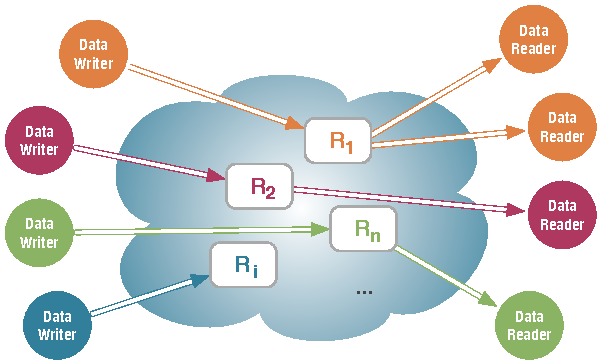
\includegraphics[scale=0.8]{xrce-interaction-model.pdf}
  \caption{XRCE interaction model}\label{fig:interaction-model}
\end{figure}

The reminder of this specification defines the protocol that makes it possible to implement the XRCE
data space abstraction.  This protocol supports data space implementations that are (1) based on a
network of brokers, (2) decentralised/peer-to-peer, or (3) a combination of (1) and (2).

As a result, the protocol defines how applications can discover each other, how application can
declare their interests and how they can share data.

\chapter{Message Notation and Serialization}

\subsection{Notation}

XRCE messages are defined using a very small domain-specific language.  The primary reason for using
a DSL is to efficiently and unambiguously describe the way header flags are used to elide
discriminators in discriminated records.  The only primitive types are natural numbers and
bytes. The natural numbers are serialised using variable length encoding, whereas bytes are
serialised unchanged.  The language specification allows any number of definitions to be
concatenated, in this document we will present individual definitions that together constitute the
full set of definitions for XRCE messages.

\begin{grammar}
  <definitions> ::= <definition> \alt <definition> <definitions>
  
  <definition> ::= <identifiers> `=' <type>

  <identifiers> ::= <identifier> \alt <identifier> `,' <identifiers>
\end{grammar}

All identifiers in the lhs of a definition are defined to be of the type specified as the rhs.

\begin{grammar}
  <type> ::= <identifier> \alt `nat' \alt `byte' \alt <sequence> \alt <header> \alt <flag> \alt <enum> \alt <record> \alt <case> \alt <option>

  <sequence> ::= `[' <type> `]'
\end{grammar}

A \emph{sequence} is a (possibly empty) list of any type other than a \emph{flag}. Serialisation of
a list is the length serialised as a natural number followed by the serialisation of the elements of
the list.

\begin{grammar}
  <header> ::= `header' <nat> <type>
\end{grammar}

A \emph{header} contrains \emph{type} to a byte or an enumerated type.  The value must be
$< 2^{nat}$.  A header is always serialised as a single byte.

\begin{grammar}
  <flag> ::= `flag' <nat>
\end{grammar}

A \emph{flag} is a boolean that is serialised by adding $2^{nat}$ to the nearest preceding header
iff true.  The position must be available (hence a sequence of flags is impossible).

\begin{grammar}
  <enum> ::= `enum' `{' <symbols> `}'

  <symbols> ::= <symbol> \alt <symbol> `,' <symbols>
  
  <symbol> ::= <identifier> `=' <nat>
\end{grammar}

An enumerated type defines a bijective mapping of symbols to natural numbers.  It is serialized as a
natural number, except when used as a header.
  
\begin{grammar}
  <record> ::= `record' `{' <member> \{ `,' <member> \} `}'

  <member> ::= <identifier> `:' <type>
\end{grammar}

A record is a product type, serialised by concatenating the serialised forms of its constituing
types.
  
\begin{grammar}
  <case> ::= `case' <identifier> `of' `{' <cases> `}'
  
  <cases> ::= <labels> $\rightarrow$ <type>
  
  <labels> ::= <label> \alt <label> `,' <labels>
  
  <label> ::= <identifier> \alt <nat> [ `...' <nat> ]
\end{grammar}

The members of a record may be sum types, where the discriminator is specified explicitly as a
preceding member of the containing record.  It is serialised by serialising the case selected by the
discriminator; if no case matches the discriminator, nothing is serialised.  E.g.:
\begin{verbatim}
record {
  a: header 5 enum { x = 1, y = 2, z = 3 },
  b: flag 5,
  c: case b of { true -> record { d: flag 6, e: nat } }
}
\end{verbatim}
serialises to a one-byte header of which the least significant 5 bits are used for encoding the
enumerated type, and where bit 5 is used to encode $b$.  If $b$ is false, that is all; if $b$ is
true, however, bit 6 of this header byte is used to encode the value of $d$, and the header byte is
followed by the value of $e$ in variable-length encoding.

\begin{grammar}
  <option> ::= `if' <type> `then' <type>
\end{grammar}

This is syntactic sugar for:
\begin{verbatim}
record { present: A, value: case A of { true -> B } }
\end{verbatim}
where A is the first \emph{type} and B the second.

\subsection{Variable-length encoding}

Natural numbers are serialised using variable-length encoding, the number $n$ is serialised as a sequence of bytes $128 + s_0, 128 + s_1, \ldots{}, 128 + s_{k-1}, s_k$

\[
  n = \sum_{i=0}^k 2^{7i}s_i \wedge 0 \leq s_i < 128 \wedge k = \left. \begin{cases}
      0, & \text{for } n = 0 \\
      \lceil (\log_2 n)/7 \rceil, & \text{for } n > 0
      \end{cases} \right.
\]

\subsection{Strings}

Strings are simply sequences of bytes, i.e.:
% MSG
\begin{verbatim}
string = [byte]
\end{verbatim}

\subsection{Header}

An XRCE message is composed of a single byte header and a body:
\begin{verbatim}
 7 6 5 4 3 2 1 0
+-+-+-+-+-+-+-+-+
|X|X|X|MessageId|
+---------------+
~      body     ~
+---------------+
\end{verbatim}
Any flag field that is not defined shall always be set to zero in outgoing messages, and shall be
ignored in received messages.
% MSG
\begin{verbatim}
Message = record {
  kind: header 5 MessageId,
  body: case kind of {
    ScoutId       -> Scout,
    HelloId       -> Hello,
    OpenId        -> Open,
    AcceptId      -> Accept,
    CloseId       -> Close,
    DeclareId     -> Declare,
    StreamDataId  -> StreamData,
    BatchedDataId -> BatchedData,
    WriteDataId   -> WriteData,
    PullId        -> Pull,
    PingId        -> Ping,
    PongId        -> Pong,
    SynchId       -> Synch,
    AckNackId     -> AckNack,
    KeepAliveId   -> KeepAlive,
    FragId        -> Frag,
    ConduitId     -> Conduit
  }
}

MessageId = enum {
  ScoutId           = 1,
  HelloId           = 2,
  OpenId            = 3,
  AcceptId          = 4,
  CloseId           = 5,
  DeclareId         = 6,
  StreamDataId      = 7,
  BatchedDataId     = 8,
  WriteDataId       = 9,
  -- QueryId        = 10,
  PullId            = 11,
  PingId            = 12,
  PongId            = 13,
  SynchId           = 14,
  AckNackId         = 15,
  KeepAliveId       = 16,
  -- ConduitCloseId = 17,
  FragId            = 18,
  ConduitId         = 19
  -- MigrateId      = 20,
  -- StreamDeltaId  = 21,
  -- BatchedDeltaId = 22,
  -- WriteDeltaId   = 23
}
\end{verbatim}

The header flags have single-letter names, but to let these letters be mnemonic, each flag has
several names depending on context:
% MSG
\begin{verbatim}
S, M, P, L = flag 5
C, R, H, N = flag 6
Z, A, U, G = flag 7
\end{verbatim}

Their (primary) use is as outlined in the below table, for easy reference.  For the definitions, see
the message definitions that use them.  The Z, L and H flags are odd ones and used only for Conduit
message.

\begin{tabu}{llX}
  flag & name       & interpretation \\ \hline
  S    & sync       & used in reliable messages to request a prompt acknowledgement \\
  M    & mask       & presence of a mask in an acknowledgement \\
  P    & properties & presence of properties in the message \\
  C    & committed  & a set of declarations that has already been committed \\
  R    & reliable   & indicates that the message is reliable \\
  N    & number     & the presence of a count \\
  A    & actual     & an ``actual'' resource id is present in the contents of a data set \\
  U    & unacked    & count of messages available for retransmission \\
  G    & global     & indicates the selection id is globally unique \\
\end{tabu}

\subsection{Properties}

A property is a pair of a numerical id and a octet sequence as value.  Properties are always
optional, their presence indicated by the P flag:
% MSG
\begin{verbatim}
Property   = record {
  id: nat,
  value: [byte]
}
Properties = if P then [Property]
\end{verbatim}

Even property ids are reserved for standardised properties, odd ones are reserved for
vendor-specific properties.  The standardised properties and their values are as follows, where the
specified value shall be a prefix of the ``value'' sequence of octets:

\begin{tabu}{rX}
  id & interpretation \\ \hline
   0 & vendor id a DDSI vendor code in DDSI encoding (default is an unspecified vendor) \\
   2 & maximum number of conduits (that is, highest supported conduit id + 1), VLE encoded (default is 1) \\
   4 & sequence number length in bits, VLE encoded (default is 14) \\
   6 & reliability flag, either 1 for reliable, or 0 for unreliable (default is 1, reliable) \\
   8 & durability flag, either 0 for volatile, 1 for transient, or 2 for persistent (default is 0, volatile) \\
  10 & commit mode, the number of pending declarations in VLE encoding that the sender can handle while processing a COMMIT message. When 0, no declarations may be sent to it following a COMMIT until after the corresponding RESULT has been received; when 1, one may continue, but must stop at the 2nd COMMIT until after a RESULT for the first COMMIT has been received; \&c. \\
  12 & authentication data \ldots{} \\
  14 & client hash \ldots{} \\
\end{tabu}

\subsection{Locators}

Locators are ... udp/A.B.C.D:PORT ...
% MSG
\begin{verbatim}
Locator = string
\end{verbatim}


%%%%%%%%%%%%%%%%%%%%%%%%%%%%%%%%%%%%%%%%%%%%%%%%%%%%%%%%%%%%%%%%%%%%%%%%%%%%%%%%%%%%%%%%%%%%%%%%%%%%%%%%%%%%%

\section{Scouting}

Scouting is used to discover anything that may engage in an XRCE interaction, such as brokers,
services, peers, etc.  For those familiar with the DDS discovery protocol, XRCE scouting can be seen
as some kind of Participant Discovery Protocol.

\subsection{Scout Message}

A node may send a Scout message to probe responses from specific kind of nodes it is interested
in.  The Scout message has the following structure:
% MSG
\begin{verbatim}
Scout = record {
  mask: nat,
  properties: Properties
}
\end{verbatim}
Its attributes have the following meaning:
\begin{description}
\item[mask] The bitmask identifying the kind of XRCE nodes being scouted, and is unbounded.
  Implementations are required to handle at least masks $< 16384$.  the meaning of the bits of mask
  is:

  \begin{tabu}{lX}
    bit & interpretation \\ \hline
    0   & broker \\
    1   & durability \\
    2   & peer \\
    3   & client \\
    $4 \ldots{} 13$ & reserved
  \end{tabu}
\end{description}

The default address for scouting on a UDP/IPv4-based transport is udp/239.255.0.1:7447.

\subsection{Hello Message}

Upon receiving a Scout message, a node matching the scout mask shall promptly respond with a Hello
message:
% MSG
\begin{verbatim}
Hello = record {
  mask: nat,
  locators: [Locator],
  properties: Properties
}
\end{verbatim}
Its attributes have the following meaning:
\begin{description}
\item[mask] The bitmask describing the XRCE node that is sending the Hello; see the Scout message
  for additional information on the interpretation of the mask.
\item[locators] The list of locators at which this node can be reached, in addition to the source
  address of the Hello message.
\end{description}

%%%%%%%%%%%%%%%%%%%%%%%%%%%%%%%%%%%%%%%%%%%%%%%%%%%%%%%%%%%%%%%%%%%%%%%%%%%%%%%%%%%%%%%%%%%%%%%%%%%%%%%%%%%%%

\section{Session Management}

Once scouting has resulted in the discovery of other nodes, or alternatively if scouting information
is configured statically, an XRCE node can start establishing sessions with the entities with which
it wishes to interact.  An XRCE session is characterized by the state machine depicted in
Figure~\ref{fig:session-initiator}.  A newly started application does not have any session, thus
starts in the closed session state.  The session management protocol is then used to open as well
close sessions.

\begin{figure}
\centering
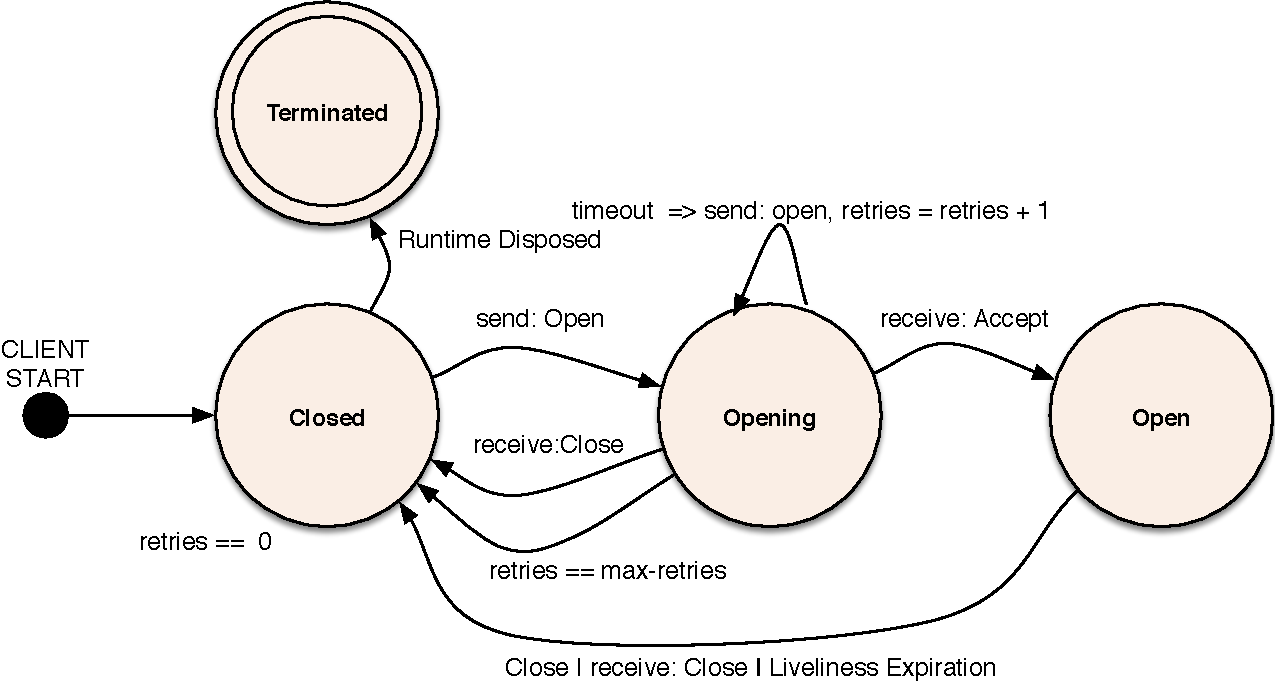
\includegraphics[scale=0.4]{session-initiator.pdf}
\caption{Session management state machine for the session initiator}\label{fig:session-initiator}
\end{figure}

\begin{figure}
\centering
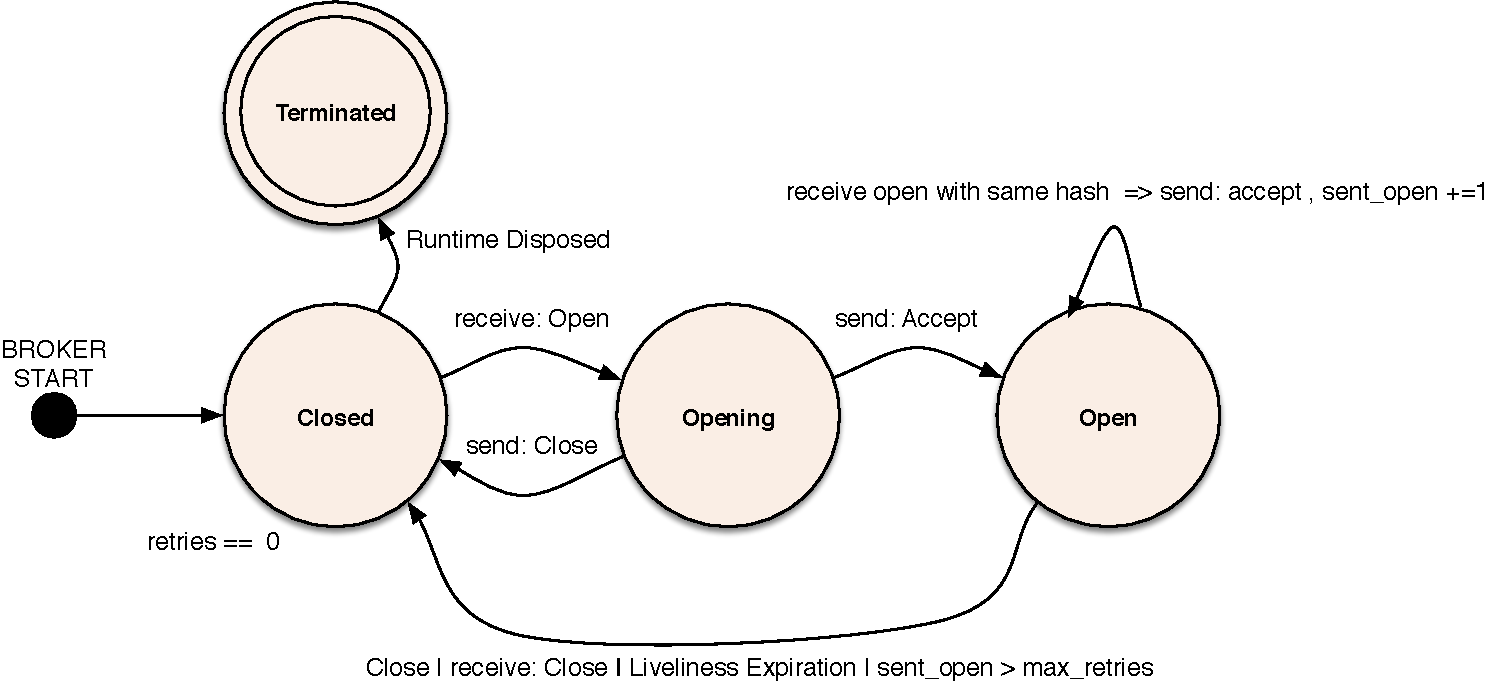
\includegraphics[scale=0.4]{session-acceptor.pdf}
\caption{Session management state machine for the broker}\label{fig:session-acceptor}
\end{figure}

\subsection{Session Establishment}

The protocol exchange for opening a session between an XRCE entities is described in the sequence
diagram described in Figure~\ref{fig:open-session}.  As represented in
Figure~\ref{fig:open-session}a, to establish a session an XRCE application sends an Open message to
the broker which in turn responds with an Accept if the section can be established or with a Close
otherwise (see Figure~\ref{fig:open-session}b).

\begin{figure}
\centering
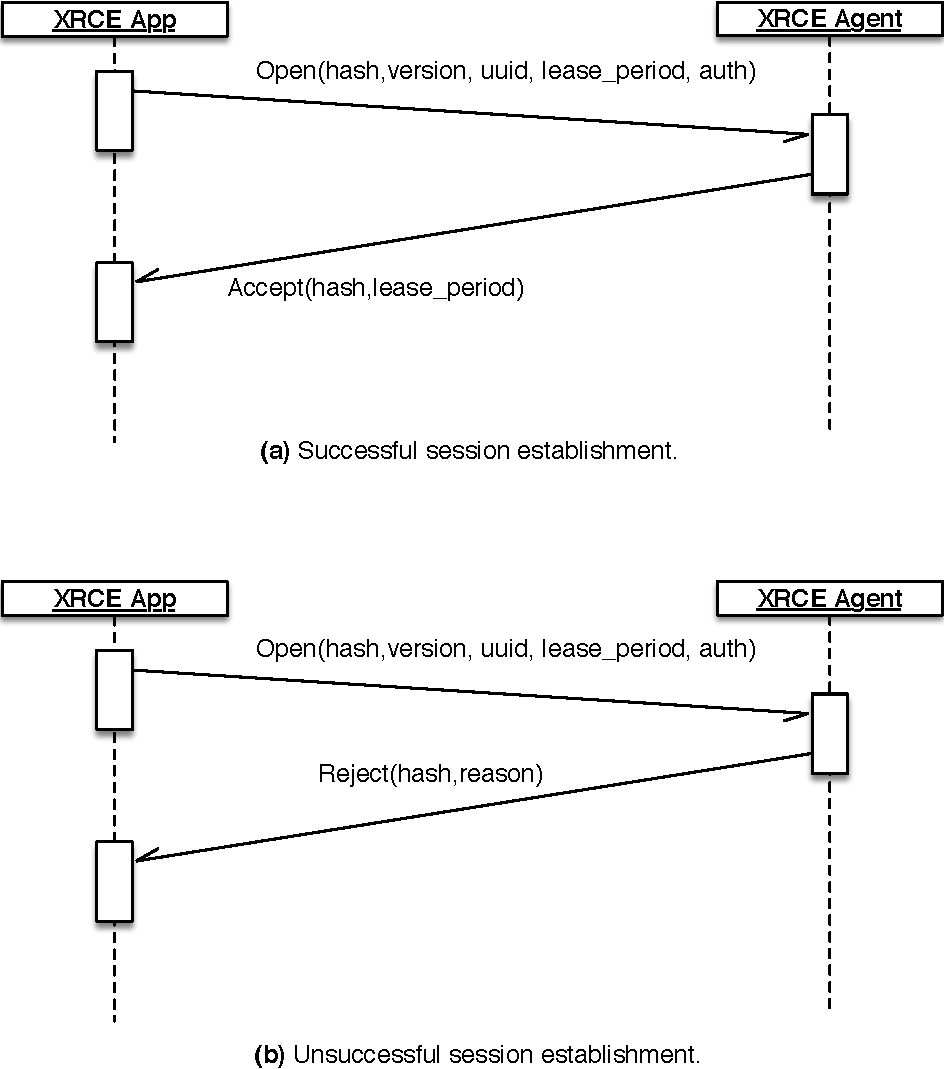
\includegraphics[scale=0.6]{open-session.pdf}
\caption{Successful session establishment}\label{fig:open-session}
\end{figure}

The Open message is sent with best effort reliability.  As a consequence, an XRCE application should
resend an Open for which no Accept or Close has been received after a configurable timeout.
Likewise, the Accept and the Close messages are also sent with best effort reliability.  Thus, an
Accept should be resent --- up to a configurable maximum number of times --— for session that have
been already accepted each time a request is received by the broker.

The sequence number size is negotiated, that is, the Open message contains a requested sequence
number size, and the recipient of the open message shall reject the session if it can’t handle the
requested sequence number size.  The negotiated sequence number size is denoted by snsize.

\subsubsection{Open Message}

The Open message has the following structure:
% MSG
\begin{verbatim}
Open = record {
  version: byte,
  pid: [byte],
  lease: nat,
  locators: [Locator],
  properties: Properties
}
\end{verbatim}
Its attributes have the following meaning:
\begin{description}
\item[version] The protocol version.
\item[pid] The participant id, a sequence of bytes that is unique within the scope of the
  application.  Implementations are required to accept at a minimum ids of at least 1 byte and at
  most 16 bytes in length.
\item[lease] This is the period --- expressed in hundreds of milliseconds --- for which the accepting
  party should assume the application is alive, even if no traffic has been received. A lease period
  of 0 (zero), represents an infinite lease.  There is no specified upper bound to a valid lease
  duration, but implementations are allowed to impose an arbitrarily chosen bound for a finite
  lease.  If the specified lease duration is larger than the upper bound for the finite lease, the
  session shall be rejected with the appropriate error code (cf.\  the Close message)
\item[locators] The list of locators at which this node can be reached, in addition to the source
  address of the Open message.
\end{description}

\subsubsection{Accept Message}

The Accept message has the following structure:
% MSG
\begin{verbatim}
Accept = record {
  openPid: [byte],
  acceptPid: [byte],
  lease: nat,
  properties: Properties
}
\end{verbatim}
Its attributes have the following meaning:
\begin{description}
\item[openPid] The id of the participant that sent the open message.
\item[acceptPid] The id of the participant that is accepting the session.
\item[lease] See the lease field of the Open message.
\end{description}

\subsection{Session Termination}

The protocol exchange for gracefully closing a session between an XRCE application and a broker is
described in the sequence diagram described in Figure~\ref{fig:close-session}.  As represented in
Figure~\ref{fig:close-session}, to close a session an XRCE application (broker) sends a Close message
to the broker (application) which in turn, when ready to close the session, responds with a Close.
Notice that implementations that decide not to wait for the matching close may end up losing data.
A session is implicitly closed after the expiration of the lease period.
 
\begin{figure}
\centering
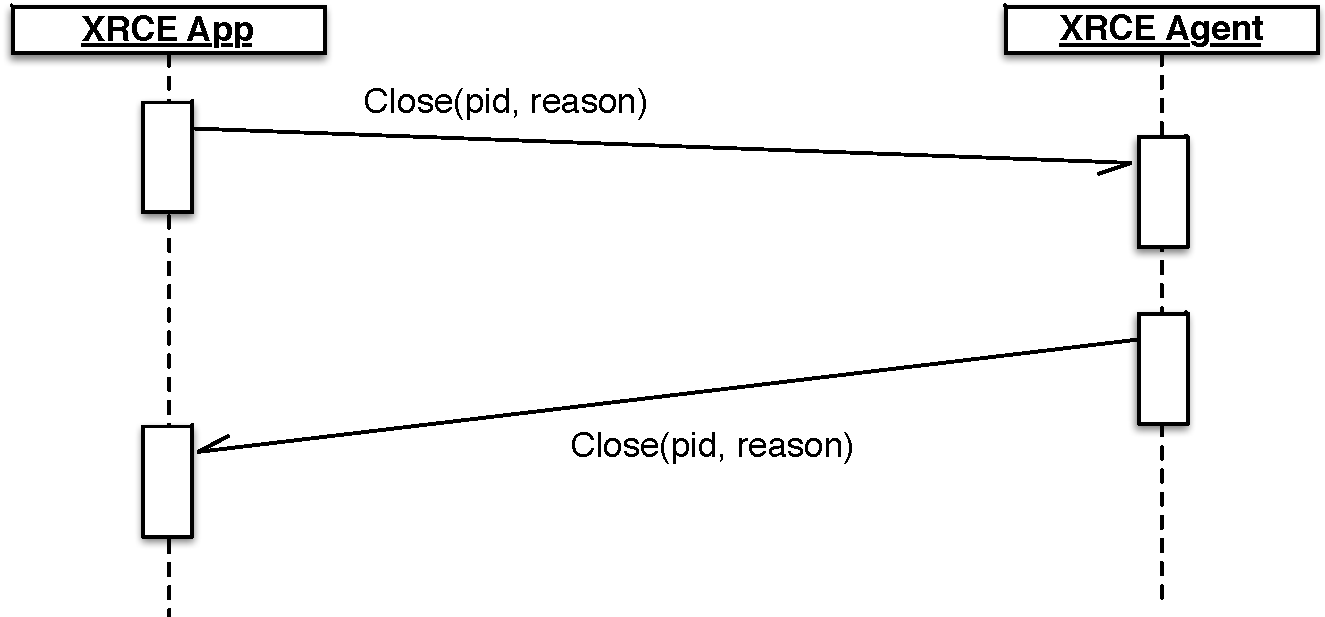
\includegraphics[scale=0.6]{close-session.pdf}
\caption{Session termination}\label{fig:close-session}
\end{figure}

\subsubsection{Close Message}

The Close message has the following structure:
% MSG
\begin{verbatim}
Close = record {
  pid: [byte],
  reason: byte
}
\end{verbatim}
Its attributes have the following meaning:
\begin{description}
\item[pid] The pid of the peer closing the session (or rejecting the opening of a session).
\item[reason] The reason why the session is being closed/rejected.  Predefined codes for Reason are:

  \begin{tabu}{rX}
    reason & meaning \\ \hline
      0 & success \\
      1 & invalid authentication data \\
      2 & unsupported protocol (version) \\
      3 & out of resources \\
      4 & unsupported sequence number length \\
      5 & unsupported parameter (e.g., lease, locators, peer id, subscription mode) \\
      6 & incompatible pre-committed declaration \\
    255 & generic error \\
    \end{tabu}
    Error codes in the range $[64,254]$ are reserved for vendor-specific error codes.\footnote{Note that on a two's complement machine, this means any codes less than -1 when the octet is interpreted as a signed 8-bit number are vendor-specific — as are any negative ones on a ones' complement machine.}
\end{description}

\subsection{Session Liveliness}

The session is kept alive as far as there is at least a protocol message sent per lease period.  If
the lease expires without the reception of any message, the session loses its liveliness.  The timed
state machine of Figure~\ref{fig:lease-expiration} describes the operations of the liveliness
protocol.

\begin{figure}
\centering
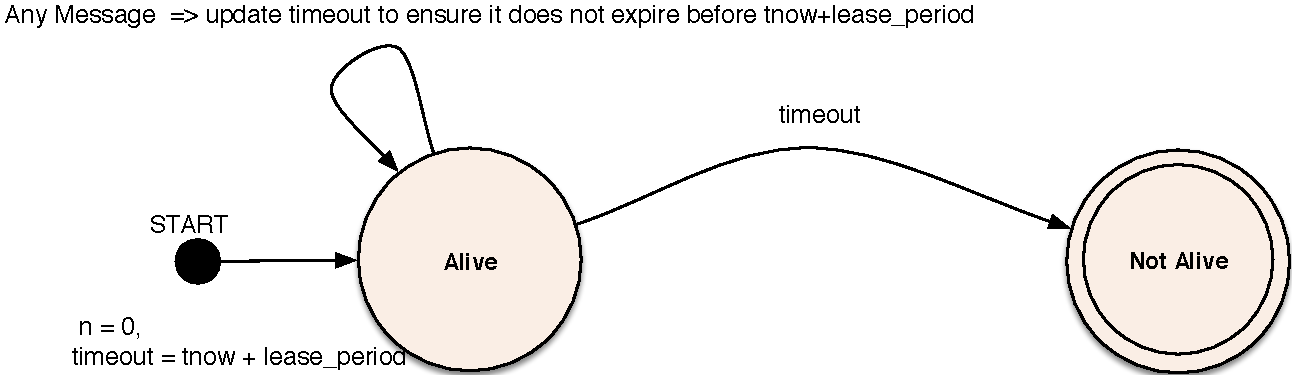
\includegraphics[scale=0.4]{lease-expiration.pdf}
\caption{Liveliness state machine}\label{fig:lease-expiration}
\end{figure}

As indicated by the liveliness state machine any protocol message renews the lease, that said it is
important to remark that when two entities communicate there are two sides of the session that need
to be maintained.

\subsubsection{KeepAlive Message}
A session lease can be renewed explicitly by sending a KeepAlive message defined as follows:
% MSG
\begin{verbatim}
KeepAlive = record {
  pid: [byte]
}
\end{verbatim}
Its attributes have the following meaning:
\begin{description}
\item[pid] The pid of the peer wants to renew the lease.
\end{description}

%%%%%%%%%%%%%%%%%%%%%%%%%%%%%%%%%%%%%%%%%%%%%%%%%%%%%%%%%%%%%%%%%

\subsection{Session Endpoints}

Now that we have specified how a session can be established and torn-down, we need define how the
endpoints of a session are identified and what is associated with a session.  From a broker
perspective an application session is represented by the tuple (pid, locators), where the pid is the
unique identifier of the participant while the locators are the set of locators received from
participant pid in the hello and/or open messages, augmented with the source address of the latest
received message from that participant that contained its pid.  In essence, a client application can
open a session across multiple transports and networks (such as TCP/IP, UDP/IP) but use all of those
transport session to carry on in the most optimal manner communication between the client and the
broker.

Notice that the locators uniquely identify a participant/client session.  That means that multiple
participant/client sessions cannot be multiplexed on the same connection.  This is not a limitation
since a client session is associated with a Domain Participant, but all the reader/writer traffic
associated with a domain participant will be multiplexed across the transport connection belonging
to the session.  Finally, it is worth pointing out that typically DDS applications have a single
domain participant per domain, thus constraining a session to a participant is not introducing any
limitation.

\subsection{Entity Declaration}

Once a session has been established, entities such as resources, publisher and subscribers can be
declared.  To maintain entity declaration atomic while ensuring that messages can be kept small,
XRCE has a concept of commit for declarations.  In other terms, declarations are taken into account
only after a commit is received.  The result of the declaration is provided back to inform the
sender of the declarations whether the declarations have been accepted or not.

\subsubsection{Resource and Selection Identifiers}

Throughout the specification, numerical resource and selection identifiers are used.  Resource
identifiers are positive even numbers and selection identifiers are positive odd numbers.  There is
no specified upper bound for resource or selection identifiers, but it is recommended that general,
interoperable implementations provide support for identifiers in $1 \ldots{} 2^{63}-1$.

Whenever an identifier is required in a declaration but the identifier does not have to correct form
or is out of bounds for the implementation, the declaration shall be rejected.

\subsubsection{Declare Message}

The message used to declare entities has the following format:
% MSG
\begin{verbatim}
Declare = record {
  sync: S,
  committed: C,
  sn: nat,
  declarations: [Declaration]
}
\end{verbatim}
Its attributes have the following meaning:
\begin{description}
\item[sync] iff set, asks for receiving an ack immediately. 
\item[committed] iff set indicates that the contained declarations have already been committed to by
  the sender and are not part of a transaction, and that the recipient shall close the session if it
  would otherwise reject some of the contained declarations.
\item[sn] The sequence number of this message
\item[declarations] A sequence of declarations (see following subsections).
\end{description}

The Declare message is always sent over the reliable channel.

\subsubsection{Declarations}

As we saw above, a Declare message contains a sequence of declarations.  Similar to messages, the
wire format of each declaration begins with a header of one octet encoding the kind as well as a
number of flags.  Again, like in messages, undefined flags shall be set to 0 in outgoing
declarations, and shall be ignored in received declarations.

% MSG
\begin{verbatim}
Declaration = record {
  kind: header 5 DeclarationId,
  declaration: case kind of {
    ResourceDeclId         -> ResourceDecl,
    PublisherDeclId        -> PublisherDecl,
    SubscriberDeclId       -> SubscriberDecl,
    SelectionDeclId        -> SelectionDecl,
    BindingDeclId          -> BindingDecl,
    CommitDeclId           -> CommitDecl,
    ResultDeclId           -> ResultDecl,
    ForgetResourceDeclId   -> ForgetResourceDecl,
    ForgetPublisherDeclId  -> ForgetPublisherDecl,
    ForgetSubscriberDeclId -> ForgetSubscriberDecl,
    ForgetSelectionDeclId  -> ForgetSelectionDecl
  }
}

DeclarationId = enum {
  ResourceDeclId         = 1,
  PublisherDeclId        = 2,
  SubscriberDeclId       = 3,
  SelectionDeclId        = 4,
  BindingDeclId          = 5,
  CommitDeclId           = 6,
  ResultDeclId           = 7,
  ForgetResourceDeclId   = 8,
  ForgetPublisherDeclId  = 9,
  ForgetSubscriberDeclId = 10,
  ForgetSelectionDeclId  = 11
}
\end{verbatim}

\paragraph{Resource Declaration.} The resource declaration corresponds to the ResourceDeclId clause
in the Declaration type defined above.
% MSG
\begin{verbatim}
ResourceDecl = record {
  rid: nat,
  resource: string,
  properties: Properties
}
\end{verbatim}
The attributes of this declaration have the following meaning:
\begin{description}
\item[rid] the numerical identifier of the resource.
\item[resource] the URI defining the resource, notice that this is one of the few messages in which
  the name of the resource appears, almost everywhere else the resource id is used to save space and
  allow to bound the message size.
\item[properties] optional properties associated with the resource; the P flag shall be set iff
  properties are present in the message.
\end{description}
Notice that resources are immutable, that means once declared it cannot be mutated. Finally resource
declaration is idempotent.

\paragraph{Publisher Declaration.} The publisher declaration corresponds to the PublisherDeclId
clause in the Declaration type defined above.
% MSG
\begin{verbatim}
PublisherDecl = record {
  rid: nat,
  properties: Properties
}
\end{verbatim}
The attributes of this declaration have the following meaning:
\begin{description}
\item[id] the numerical identifier of the resource or of the selection.  properties: optional
  properties associated with the publisher; the P flag shall be set iff properties are present in
  the message.
\end{description}

\paragraph{Subscriber Declaration.} The subscriber declaration corresponds to the SubscriberDeclId
clause in the Declaration type defined above.
% MSG
\begin{verbatim}
SubscriptionModeId = enum {
  PushModeId         = 1,
  PullModeId         = 2,
  PeriodicPushModeId = 3,
  PeriodicPullModeId = 4
}

SubscriberDecl = record {
  id: nat,
  mode: SubscriptionModeId,
  params: case mode of {
    PeriodicPushModeId, PeriodicPullModeId -> record {
      temporalOrigin: nat, period: nat, duration: nat
    }
  },
  properties: Properties
}
\end{verbatim}
The attributes of this declaration have the following meaning:
\begin{description}
\item[id] the numerical identifier of the resource or of the selection.
\item[mode] indicates the mode in which this subscriber wishes to receive data. Supported modes are:
  \begin{description}
  \item[PushModeId] updates shall be pushed to this subscriber;
  \item[PullModeId] data shall be stored until the subscriber pulls it (using PULL messages);
  \item[PeriodicPushModeId] updates shall be stored and pushed periodically, with the push occurring
    in the intervals [temporalOrigin + n * period, temporalOrigin + n * period + duration), n = 0,
    1, 2, …
  \item[PeriodicPullModeId] updates shall be stored until the subscriber pulls it, where the pulling
    occurs in the intervals [temporalOrigin + n * period, temporalOrigin + n * period + duration), n
    = 0, 1, 2, …  The temporalOrigin, period and duration fields are in
    milliseconds. Implementations shall support at least a period and duration of 214ms, and
    duration shall be less than period.
  \end{description}
\item[properties] optional properties associated with the publisher; the P flag shall be set iff
  properties are present in the message.
\end{description}

\paragraph{Selection Declaration.} The Selection declaration corresponds to the SelectionDeclId
clause in the Declaration type defined above.
% MSG
\begin{verbatim}
SelectionDecl = record {
  global: G,
  sid: nat,
  query: string,
  properties: Properties
}
\end{verbatim}
The attributes of this declaration have the following meaning:
\begin{description}
\item[sid] the numerical identifier of the selection.  This identifier can be locally generated and
  specific to a runtime or global.  As discussed next, a binding mechanism is provided to agree a
  common selection id between different nodes.
\item[query] the string representing the predicate associated with this selection.
\item[properties] optional properties associated with the publisher.
\item[global] when true indicates that sid is a global selection id.
\end{description}

\paragraph{Binding Declaration.} The Binding declaration is used to change the id associated with a
selection, this is typically done with a selection has associated multiple local id and the broker
want to be able to multicast data belonging to the selection to the interested parties.
% MSG
\begin{verbatim}
BindingDecl = record {
  global: G,
  oldId: nat,
  newId: nat
}
\end{verbatim}
The attributes of this declaration have the following meaning:
\begin{description}
\item[oldId] the old id of the selection.
\item[newId] id for the selection to be bound/aliased with the old id.
\item[global] when true indicates that newId is a global selection identifier.
\end{description}

\paragraph{Commit Declaration.} The Commit declaration is used to indicate that the receiving party
should process all the received declaration as an atomic unit.  In other terms, received
declarations are not evaluated until a commit is received and then they either all succeed, or none
of them succeed.
% MSG
\begin{verbatim}
CommitDecl = record {
  commitId: byte
}
\end{verbatim}
The attributes of this declaration have the following meaning:
\begin{description}
\item[id] the identifier associated with this transaction.
\end{description}
Whenever a commit declaration is included in a sequence of declarations, it shall be the last.

\paragraph{Result Declaration.} The Result declaration is used to communicate the result of
applying a lot of declarations.
% MSG
\begin{verbatim}
ResultDecl = record {
  commitId: byte,
  status: byte,
  id: case status of { 1 ... 255 -> nat }
}
\end{verbatim}
The attributes of this declaration have the following meaning:
\begin{description}
\item[commitId] the identifier of the commit for which this a result.
\item[status] the result of the declaration, where zero represent a success while a non-zero value
  represents an error.
\item[id] the optional id of a resource or selection included in the current transaction whose
  declaration failed.  The id field shall be omitted iff status = 0.
\end{description}

\paragraph{ForgetResource Declaration.} The forget resource declaration informs the receiver that,
as far as the sending node is concerned, the specified resource with the specified id may be removed
from the system.
% MSG
\begin{verbatim}
ForgetResourceDecl = record {
  rid: nat
}
\end{verbatim}
The attributes of this declaration have the following meaning:
\begin{description}
\item[rid] the numerical identifier of the resource.
\end{description}

\paragraph{ForgetPublisher Declaration.} The forget publisher declaration informs the receiver that
the sender will no longer be publishing for the specified resource or selection id.
% MSG
\begin{verbatim}
ForgetPublisherDecl = record {
  id: nat
}
\end{verbatim}
The attributes of this declaration have the following meaning:
\begin{description}
\item[id] the numerical identifier of the resource or selection.
\end{description}

\paragraph{ForgetSubscriber Declaration.} The forget subscriber declaration informs the receiver
that the sender is no longer subscribed to the specified resource or selection.
% MSG
\begin{verbatim}
ForgetSubscriberDecl = record {
  id: nat
}
\end{verbatim}
The attributes of this declaration have the following meaning:
\begin{description}
\item[id] the numerical identifier of the resource or selection.
\end{description}

\paragraph{ForgetSelection Declaration.} The forget selection declaration informs the receiver that
the sender will no longer be using the specified selection.
% MSG
\begin{verbatim}
ForgetSelectionDecl = record {
  sid: nat
}
\end{verbatim}
The attributes of this declaration have the following meaning:
\begin{description}
\item[sid] the numerical identifier of the selection.
\end{description}

%%%%%%%%%%%%%%%%%%%%%%%%%%%%%%%%%%%%%%%%%%%%%%%%%%%%%%%%%%%%%%%%%%%%%%%%%%%%%%%%%%%%%%%%%%%%%%%%%%%%%%%%%%%%%

\section{Data Exchange}

As a result of a session establishment between two XRCE runtimes, a conduit composed by two logical
channels, is established, as depicted in Figure~\ref{fig:xrce-conduit}.  The two conduits’ channels
may be implemented over one or more transports, for instance the best effort channel could be
implemented over UDP/IP while the reliable channel over TCP/IP\@.  However, the mechanism provided
to implement an XRCE reliable channel doesn’t require a reliable transport.  Each conduit has a
numerical identifier, starting from zero for the default conduit.  Each of the channels belonging to
the conduit has its own sequence number.

\begin{figure}
\centering
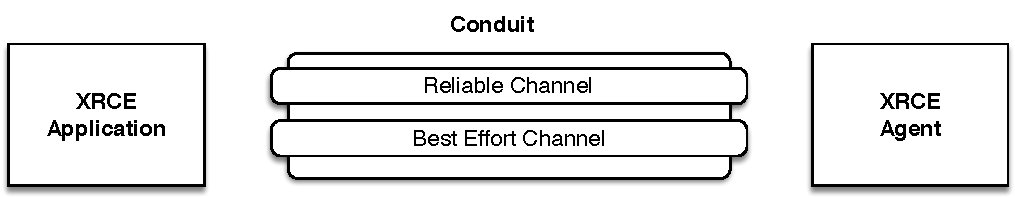
\includegraphics[scale=0.6]{xrce-conduit.pdf}
\caption{Logical communication channels between the XRCE application and the broker}\label{fig:xrce-conduit}
\end{figure}

Message exchanges that take place before successfully establishing a session are best effort.  Once
the session is established, messages that can be either best-effort or reliable use a header flag R
to discern between best-effort R=0 and reliable R=1.

\subsection{Conduits}

As explained above, as soon as a session is established the default conduit is available along with
its two channels, one reliable the other best effort.  The conduit concept allows creating another
pair of channels with their own sequence numbers that can be used to either unicast or multicast
data.  The conduit associated with a message is identified by a message marker.  This message marker
has the following structure:
% MSG
\begin{verbatim}
Conduit = record {
  compact: Z,
  id: case compact of {
    false -> nat,
    true  -> record { id1: H, id0: L }
  }
}
\end{verbatim}
The id attribute represents the conduit identifier.

If ``compact'' is true, that the compact format is used and in this case (as specified by the
Conduit message format above), there is no id following the header, but rather the H and L flags are
used to represent a conduit id: $1 + l + 2h$ where $l = 0$ if ``id0'' is false and 1 if it is true
(analogously for $h$ and ``id1'').  The compact representation is an optimisation and
implementations are free to always set ``compact'' to false and include the conduit id as a separate
value.  This takes just an additional byte --- but when you have an MTU of 20 bytes even a single
byte matters!

The highest supported conduit id is implementation-defined, and messages received on a conduit with
an unsupported conduit id shall result in closing the session.

As a final remark, recall that the conduit marker is prepended to messages that are sent over a
conduit whenever the target conduit is different from the default, conduit id 0.  Message markers,
as the name suggest, are sent as if they were a decoration of the message, thus a message and its
markers are always sent as a unit.

\subsection{Best-Effort Channel}

\subsubsection{Channel Specification}

The Best-Effort Channel supports the following primitives:
\begin{description}
\item[send] Channel $\times$ Msg $\rightarrow$ Channel
\item[receive] Channel $\rightarrow$ Msg The semantic of the channel operations are as follows:
  send: given a sequence of messages $m_0, m_1, \ldots{}, m_k$, sent over the channel, using the
  channel primitive send, the channel shall deliver an ordered subsequence:
  $m_{s_0},m_{s_1}, \ldots{} ,m_{s_h}$ where:
  \[
    \left.
      \begin{cases}
        s_0 < s_i < \ldots{} < s_h \\
        s_i \in \{ x \in \mathbb{N}_0 : 0 \leq x \leq k \}
      \end{cases}
    \right.
  \]
  In other terms, the XRCE best-effort channel may drop messages but always deliver messages in
  order. To maintain ordering the channel relies on a sequence number. The sequence number sn is
  initialized to zero at the creation of the channel and is incremented by one for every message
  sent on the channel.
\item[receive] returns a message, previously sent on the other end of this channel, if
  available. Otherwise it returns nothing.
\end{description}

\subsubsection{Channel Implementation}

The best-effort channel implementation is relatively straight forward. The XRCE runtime has to make
a reasonable effort to send the message over the associated transport and ensure that messages,
whilst may be dropped, shall never be delivered to receive out of order.

\subsection{Reliable Channel)}

\subsubsection{Channel Specification}
The Reliable Channel supports the following primitives:
\begin{description}
\item[rsend] Channel $\times$ Msg $\rightarrow$ Channel
\item[rreceive] Channel $\rightarrow$ Msg
\end{description}
The semantic of the channel operations are as follows:
\begin{description}
\item[open] creates a new Reliable Channel;
\item[close] closes the channel, in other terms no messages can be sent anymore over it;
\item[send] given a sequence of messages $m_0, m_1, \ldots{}, m_k$ sent over the channel using the
  rsend primitive, the channel will deliver (on the other end) exactly the sequence:
  \[
    m_0, m_1, \ldots{}, m_k
  \]
  In other terms, the XRCE reliable channel shall not drop messages nor deliver them out of order.
  This behaviour has to be guaranteed only under the assumption that the communicating parties are
  correct, i.e., don't fail.  To maintain ordering the channel relies on a sequence number.  The
  sequence number \emph{sn} is initialized to zero at the creation of the channel and is incremented
  by one for every message sent on the channel.
\item[receive] returns a message, previously sent on the other end of this channel, if
  available.  Otherwise it returns nothing.
\end{description}  

\subsubsection{Channel Implementation}

The Petri Net in Figure~\ref{fig:reliable-channel} describes the behaviour of a Reliable Channel
with a buffer of $n$ places.  It is worth to mention that the specification in
Figure~\ref{fig:reliable-channel} assumes that a NACK can only be received for the head of the
queue.  This may seem a restriction, but in reality it only means that when receiving a NACK for
message with sequence number $k$ the previous messages have been acknowledged.

\begin{figure}
\centering
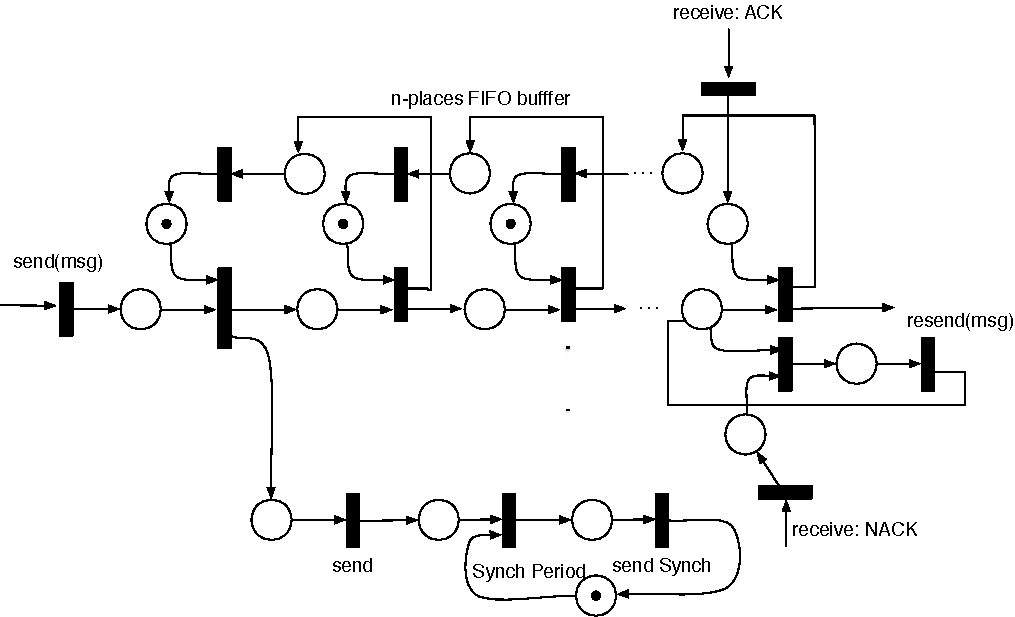
\includegraphics[scale=0.6]{xrce-relchan.pdf}
\caption{Petri Net describing the Reliable Channel behaviour}\label{fig:reliable-channel}
\end{figure}

\subsubsection{Synch Message}

Synch messages are sent on a newly created reliable channel to set the initial sequence number.  If
a synch message is not received, then zero should be considered as the first sequence number for the
reliable channel.  Synch message are sent when needed to inform the other end of the channel of the
sequence number of the latest message sent.  This allows the other end to detect message loss
without necessarily waiting for another regular message.  The structure of the synch message is:
% MSG
\begin{verbatim}
Synch = record {
  reliable: R,
  sync: S,
  sn: nat,
  count: if U then nat
}
\end{verbatim}
Where the message attributes have the following meaning:
\begin{description}
\item[reliable] set if this concerns the reliable channel, clear if it concerns the unreliable
  channel.
\item[sync] if set, the message shall be acknowledged promptly.
\item[sn] the sequence number of the next message to be transmitted on this channel
\item[count] optional number of unacknowledged messages, that is, messages with sequence numbers
  $s_{n-\mathrm{count}}, s_{n-\mathrm{count}+1}, \ldots{}, s_{n-1}$ are available for
  retransmission.  If ``count'' is absent, there are none.
  $\mathrm{Uflag} \Leftrightarrow 0 < \mathrm{count} < 2^{\mathrm{snsize}-1}-1 \wedge
  \mathrm{reliable} $.
\end{description}

\subsubsection{Positive and Negative Acknowledgements}

A single message is used to indicate both positive as well as potentially negative acknowledgements.
A node may ignore a negative acknowledgement for a message a finite number of times, but eventually,
receipt of a negative acknowledgement shall result in the retransmitting of at least the message
with sequence number sn, the oldest message for which retransmit is requested.

The structure of the message is the following:
% MSG
\begin{verbatim}
AckNack = record {
  sn: nat,
  mask: if M then nat
}
\end{verbatim}
Where the attributes have the following meaning:
\begin{description}
\item[sn] the first sequence number not received; all preceding messages are acknowledged.
\item[mask] if present, retransmission is requested for the messages
  with sequence numbers $\mathrm{sn}+i$ s.t.
  $\lfloor 2^{-i} m \rfloor - 2 \big\lfloor \lfloor 2^{-i} m \rfloor /
  2 \big\rfloor \neq 0$, where $m = 2 \mathrm{mask} + 1$.
\end{description}

The synch, positive and negative acknowledgements described in Figure~\ref{fig:reliable-channel}
shall be implemented by the messages specified before.

\subsection{Writing Data}

After a publisher has been successfully created and the declaration of a matching data reader has
been received, an XRCE implementation shall start to send data to the matching entity(s).  To avoid
any ambiguity, an XRCE runtime shall avoid to sends data on a write for writers that are not
matched.  The XRCE protocol provides different ways of ways of writing data, one which maps to that
provided by DDS\@.

\subsubsection{Write Data}

Differently from DDS, XRCE allows to write samples for resources for which a publisher was not
declared and for which only resource name is known (not the resource id).  This makes the write a
bit less wire efficient because the resource name is part of the data message, but is quite handy
for dealing with one-off writes of a resource.  These kind of writes are very cumbersome on DDS\@.

The WriteData message has the following structure:
% MSG
\begin{verbatim}
WriteData = record {
  reliable: R,
  sync    : S,
  sn      : nat,
  resource: string,
  payload : [byte]
}
\end{verbatim}
Where the attributes have the following meaning:
\begin{description}
\item[reliable] set if this concerns the reliable channel, clear if it concerns the unreliable
  channel.
\item[sync] if set, the message shall be acknowledged promptly.
\item[sn] the sequence number for this message.
\item[resource] the resource for which we are writing data.
\item[payload] the serialised data.
\end{description}
To the XRCE protocol the format of the serialised data is transparent.  Thus, when
interoperating with DDS it shall be the same as that used by DDS\@.  In stand-alone situations can
be whatever the application deems to be the most appropriate.

\subsubsection{Stream Data}

XRCE provides a very wire efficient to produce data belonging to a stream, namely the StreamData
message.  The structure of this message is as follows:
% MSG
\begin{verbatim}
StreamData = record {
  reliable: R,
  sync    : S,
  sn      : nat,
  id      : nat,
  prid    : if A then nat,
  payload : [byte]
}
\end{verbatim}
Where the attributes have the following meaning:
\begin{description}
\item[reliable] set if this concerns the reliable channel, clear if it concerns the unreliable channel.
\item[sync] if set, the message shall be acknowledged promptly.
\item[sn] the sequence number for this message.
\item[id] the matching resource/selection id for which we are writing data.
\item[prid] optionally the id of the resource to which the data belongs — this may be different to
  the matching resource/selection id for non-trivial resources and selections.
\item[payload] the serialised data.
\end{description}
Notice that the message overhead is at least 4 bytes, three bytes of protocol data and one byte --- at
minimum --- to encode the payload length.

\subsubsection{Batch Data}

XRCE supports message batching for the same resource/selection.  The BatchedData message further
improves the wire efficiency of the protocol.  The structure of this message is as follows:
% MSG
\begin{verbatim}
BatchedData = record {
  reliable: R,
  sync    : S,
  sn      : nat,
  id      : nat,
  hasPrid : A,
  payload : case hasPrid of {
    false -> [[byte]],
    true  -> [record { prid: nat, payload: [byte] }]
  }
}
\end{verbatim}
Where the attributes have the following meaning:
\begin{description}
\item[reliable] set if this concerns the reliable channel, clear if it concerns the unreliable channel.
\item[sync] if set, the message shall be acknowledged promptly.
\item[sn] the sequence number for this message.
\item[id] the matching resource /selection id for which we are writing data
\item[payload] the batched data.
\end{description}
Notice that the minimal overhead in this case is: $(3+n)/n$ which gets very quickly close to 1 as
the number $n$ of batched message grows beyond a few.

\subsection{Reading Data}

While in regular DDS reads are always local, in XRCE that is not always possible or desirable
due to memory or network constraints.  As such XRCE needs a message to pull data remotely.

\subsubsection{Pull Message}
Pull is a reliable message with the following structure:
% MSG
\begin{verbatim}
Pull = record {
  sync: S,
  sn: nat,
  id: nat,
  pullId: nat,
  maxSamples: if N then nat
}
\end{verbatim}
Its attributes have the following meaning:
\begin{description}
\item[sync] if set, the message shall be acknowledged promptly.
\item[sn] the message sequence number.
\item[id] the resource / selection id for which data has to be pulled.
\item[pullId] an id used to identify this pull session.  This way any state required can be cached
  on the broker side. Implementations at least support $0 ≤ \mathrm{pullId} < 16$.
\item[maxSamples] optionally the maximum number of samples that this node is willing to receive
  before having to issue another pull.  Implementations shall at least support
  $0 < \mathrm{maxSamples} < 2^{16}$.
\end{description}

\subsubsection{Data Fragmentation}

XRCE supports fragmentation to accommodate sending user data of any size.  This is done by a message
marker called Frag.  As in the case of the Conduit message marker, these messages have to be sent in
the same packet as the message they mark.  Fragmentation shall not be used for messages that fit in
one MTU, and whenever data is fragmented into $n > 1$ fragments, the first $n - 1$ fragments shall
have the same size and the last fragment shall be no larger than the preceding fragments.  The
structure of the Frag message is defined below:
% MSG
\begin{verbatim}
Frag = record {
  snBase: nat,
  n: if N then nat
}
\end{verbatim}
Where the attributes have the following meaning:
\begin{description}
\item[snBase] the sequence number of the first message in this series of fragment.
\item[n] if present tells the total number of fragments. Otherwise it can be deduced by looking at
  the first in order message that does not have the fragment marker.
\end{description}

\subsection{Roundtrip-Time Estimation}

Latency estimation is essential in order to do proper reliability window management.  As such the
XRCE protocol provides a couple of messages to estimate the roundtrip-time between to nodes.  These
messages are called Ping and Pong respectively and their structure is shown below.
% MSG
\begin{verbatim}
Ping = record {
  hash: nat
}
Pong = record {
  hash: nat
}
\end{verbatim}
On receipt of a Ping, a Pong with the same hash shall be sent in response.  An implementation shall
at least support hashes $< 2^{16}$.

\end{document}
